\documentclass[11pt]{article}
\usepackage{amsmath}
\usepackage{amssymb}
\usepackage{graphicx}
\usepackage{fancyhdr}
\usepackage{enumerate}
\usepackage{titlesec}
\usepackage[colorlinks=true,urlcolor=blue]{hyperref}

\titlespacing{\subsubsection}{0pt}{0pt}{0pt}

% No page numbers
%\pagenumbering{gobble}

% INFORMATION SHEET (DO NOT EDIT THIS PART) ---------------------------------------------
\newcommand{\addinformationsheet}{
\clearpage
\thispagestyle{empty}
\begin{center}
\LARGE{\bf \textsf{Information sheet\\CS224W: Analysis of Networks}} \\*[4ex]
\end{center}
\vfill
\textbf{Assignment Submission } Fill in and include this information sheet with each of your assignments.  This page should be the last page of your submission.  Assignments are due at 11:59pm and are always due on a Thursday.  All students (SCPD and non-SCPD) must submit their homeworks via GradeScope (\url{http://www.gradescope.com}). Students can typeset or scan their homeworks. Make sure that you answer each (sub-)question on a separate page. That is, one answer per page regardless of the answer length. Students also need to upload their code at \url{http://snap.stanford.edu/submit}. Put all the code for a single question into a single file and upload it. Please do not put any code in your GradeScope submissions. 
\\
\\
\textbf{Late Homework Policy } Each student will have a total of {\em two} free late periods. {\em Homeworks are due on Thursdays at 11:59pm PDT and one late period expires on the following Monday at 11:59pm PDT}.  Only one late period may be used for an assignment.  Any homework received after 11:59pm PDT on the Monday following the homework due date will receive no credit.  Once these late periods are exhausted, any assignments turned in late will receive no credit.
\\
\\
\textbf{Honor Code } We strongly encourage students to form study groups. Students may discuss and work on homework problems in groups. However, each student must write down their solutions independently i.e., each student must understand the solution well enough in order to reconstruct it by him/herself.  Students should clearly mention the names of all the other students who were part of their discussion group. Using code or solutions obtained from the web (github/google/previous year solutions etc.) is considered an honor code violation. We check all the submissions for plagiarism. We take the honor code very seriously and expect students to do the same. 
\vfill
\vfill
}
% ------------------------------------------------------------------------------

% MARGINS (DO NOT EDIT) ---------------------------------------------
\oddsidemargin  0.25in \evensidemargin 0.25in \topmargin -0.5in
\headheight 0in \headsep 0.1in
\textwidth  6.5in \textheight 9in
\parskip 1.25ex  \parindent 0ex \footskip 20pt
% ---------------------------------------------------------------------------------

% HEADER (DO NOT EDIT) -----------------------------------------------
\newcommand{\problemnumber}{0}
\newcommand{\myname}{name}
\newfont{\myfont}{cmssbx10 scaled 1000}
\pagestyle{fancy}
\fancyhead{}
\fancyhead[L]{\myfont Question \problemnumber, Problem Set 3, CS224W}
%\fancyhead[R]{\bssnine \myname}
\newcommand{\newquestion}[1]{
\clearpage % page break and flush floats
\renewcommand{\problemnumber}{#1} % set problem number for header
\phantom{}  % Put something on the page so it shows
}
% ---------------------------------------------------------------------------------


% BEGIN HOMEWORK HERE
\begin{document}

% Question 1
\newquestion{1}

\subsubsection*{(a)}
$$ N = \{ N_0, N_1, ..., N_{n-1}\}, l \in [n], N'_i := \text{Number of people already rioting before $N_i$}$$
$$ \text{Condition for\ } N_1: N'_1 \geq 1, N'_1 = N_0 \therefore N_0 \geq 1 $$ 
$$ \text{Condition for\ } N_2: N'_2 \geq 2, N'_2 = N_0 + N_1 \therefore N_0 + N_1 \geq 2 $$
Set $t=2$ and solve inductively. 
$$ \text{Condition for\ } N_t: N'_t \geq t, N'_t = N_{t-2} + N_{t-1} $$
$$ N'_t = \sum_{i=0}^{t-1} N_i $$
$$ \text{Condition for\ } N_t: \sum_{i=0}^{t-1} N_i \geq t $$
 
\subsubsection*{(b)}
First define the histogram of margins over the condition previously specified as follows, 
$$ \tilde{N_i} = \sum_{j=0}^i N_j - i, \ \tilde{N} = \{\tilde{N_1}, \tilde{N_2}, ... \} $$
Then restrict this set to values with non-positive margin, and take the instance  of the maximum, where $n^*$ is then the first time the threshold is not met, and is therefore where the spread will stop. 
$$ n^* = arg\max_i \{n_i | n_i \in \tilde{N}, n_i \leq 0 \} $$
\subsubsection*{(c)}
A total of 45 people will join the riot. This can be seen in the graph below by iterating on the histogram and curve of $x=y$. Start at $H_0$ and move horizontally to where $x = H_0$. From this point, move vertically to the histogram value at $H_x$. Repeat this process until $H_x = x$. If the histogram creates a continuous "curve", this is the point where that curve crosses $x = y$.  
\begin{center}
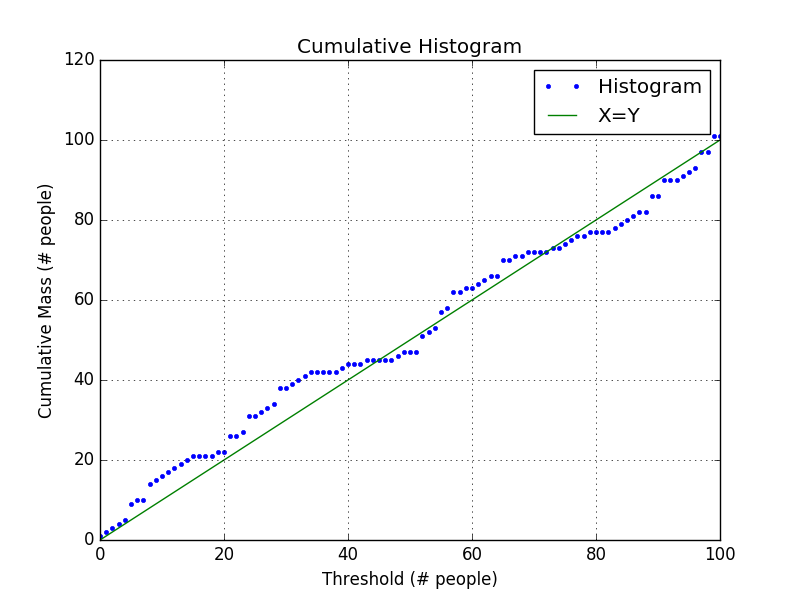
\includegraphics[scale=0.45]{P1_3.png}
\end{center}

% Question 2.1
\newquestion{2.1}
$$ P(X = x) = (\frac{\alpha - 1}{x_{min}}) (\frac{x}{x_{min}})^{-\alpha} $$
$$ P(X \geq x) = 1 - P(X \leq x) $$ 
$$ P(X \geq x) = 1 - (\frac{\alpha - 1}{x_{min}})x_{min}^\alpha \int_{x_{min}}^x t^{-\alpha} dt $$
$$ P(X \geq x) = 1 - (\alpha - 1)x_{min}^{\alpha - 1} (1 - \alpha)^{-1} [t^{1-\alpha}|_{t = x_min}^{t=x}  $$ 
$$ P(X \geq x) = 1 + x_{min}^{\alpha - 1}(x^{1 - \alpha} - x_{min}^{1 - \alpha}) $$
$$ P(X \geq x) = (\frac{x}{x_{min}})^{1 - \alpha} $$
% Question 2.2
\newquestion{2.2}
First sample from the uniform distribution, $ u ~ U[0, 1] $. Then set this value equal to the cCDF as shown below. 

$$ u = (\frac{x}{x_{min}})^{1 - \alpha} $$
$$ x = x_{min}u^\frac{1}{1 - \alpha} $$
\begin{center}
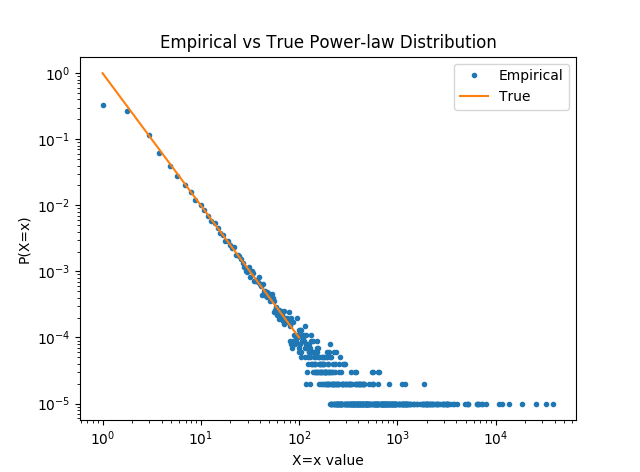
\includegraphics[scale=0.5]{P2_2.png}
\end{center}
% Question 2.3
\newquestion{2.3}
First take the log of the PDF so that the function is linear in $\alpha$.
$$ log(P) = -\alpha \log\frac{x}{x_{min}} + \log \frac{\alpha - 1}{x_{min}} $$
Then define the array of training examples $\tilde{X}$, concatenated with a constant vector of 1 (to account for the bias) such that,

$$ \tilde{X} \in \mathbb{R}^{n X 2},\ \tilde{X} = [ \log \frac{X}{x_{min}},  1 ] $$   
We can then define the problem as the affine function with the closed form solution below, with $A \in \mathbb{R}^2 $. 
$$ \tilde{X} A = \log P$$
$$ A = (\tilde{X}^T\tilde{X})^{-1}\tilde{X}^T \log P $$
From the solution of $A$, $ \alpha $ and $ x_{min} $ can be found. 
$$ A_1 = -\alpha, \ A_2 = \log \frac{\alpha - 1}{x} $$ 
Using this approach, the following values were computed: 
$$ \alpha_{LS} = 2.096, x_{min,LS} = 0.699 $$ 
As can be seen in the plot in sub-question 2.2, there are several points at the tails of the distribution that are not well aligned to the true distribution. By restricting the data considered to those points at the middle of the distribution, the influence of these noisy outliers can be reduced. In this we restricted our selection to the middle 50 points. The resulting values and graph with both curves are shown below. 
$$ \alpha'_{LS} = 1.960, x'_{min,LS} = 1.096 $$

\begin{center}
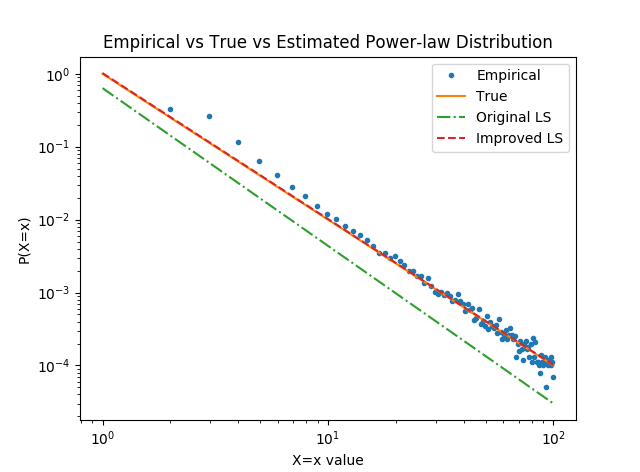
\includegraphics[scale=0.75]{P2_3.png}
\end{center}

% Question 2.4
\newquestion{2.4}
Define the log-likelihood function for the dataset
$$ l(\alpha) = \sum_{i=1}^n \log P(X=x_i ;\alpha) $$
$$ l(\alpha) = \sum_{i=1}^n[ \log \frac{\alpha - 1}{x_{min}} - \alpha \log \frac{x_i}{x_{min}}] $$
Take the derivative with respect to $\alpha$ (since we're holding $x_min$ fixed). 
$$ \frac{\partial}{\partial \alpha} l(\alpha) = \sum_{i=1}^n [ \frac{x_{min}}{\alpha - 1}\frac{1}{x_{min}} - \log \frac{x_i}{x_{min}} $$
Set this equal to 0 and solve for $\alpha$
$$ \sum_{i=1}^n \frac{1}{\alpha -1} = \sum_{i=1}^n \log \frac{x_i}{x_min} $$ 
$$ \frac{n}{\alpha -1}	= \sum_{i=1}^n \log \frac{x_i}{x_min} $$
$$ \alpha_{MLE} = \frac{n}{\sum_{i=1}^n \log \frac{x_i}{x_min}} + 1 $$
Using this method, we compute $\alpha_{MLE} = 2.045 $ 
\begin{center}
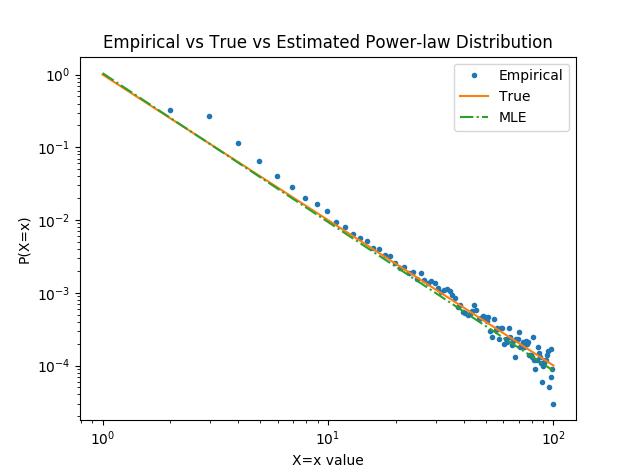
\includegraphics[scale=0.75]{P2_4.png}
\end{center}
% Question 2.5
\newquestion{2.5}
$$ \text{Mean}: \mu_{LS} = 2.136,\ \mu'_{LS} = 2.029, \mu_{MLE} = 2.046 $$
$$ \text{STD}: \sigma_{LS} = 0.0196,\ \sigma'_{LS} = 0.0139, \sigma_{MLE} = 0.0038 $$
% Question 3.1
\newquestion{3.1}

Proportion of simulations causing epidemic IMDB network: 0.0\%
Proportion of simulations causing epidemic Erdos Renyi: 85.9 \%
Proportion of simulations causing epidemic Preferential Attachment: 76.0 \%

Average infected in IMDB: 27.3 \%
Average infected in Erdos Renyi: 63.3 \%
Average infected in Preferential Attachment: 53.1 \%

Average infection in Erdos Renyi Epidemics: 73.7 \% 
Average infection in Preferential Attachment Epidemics: 69.9 \%

Results from the Chi-square tests;
$$\chi_{IMDB, ER}  = 147.39,\ p_{IMDB, ER} = 6.45e-34 $$
$$\chi_{IMDB, PA}  = 119.38,\ p_{IMDB, PA} = 8.66e-28 $$
$$\chi_{PA, ER}  = 2.63,\ p_{PA, ER} = 0.105 $$

The Erods-Renyi appears to be more succeptable to epidemics than the preferential attachment graph. We can say with ~ 90 \% confidence that this difference is not due to a random process independent from the graph structure. 

Erdos-Renyi appears to have higher final percentage infection in instances of epidemic. 

Overall, Eros-Renyi appears to be more succeptable to disease spreading than Preferential Attachment. 

I would expect a graph with greater structure and a more skewed degree distribution to be mroe resistant to disease outbreak. Based on the SIR model, the epidemic threshold for a complete graph is equal to the first eigenvalue of the graph. Therefore, networks with more degree distribution concentrated in a smaller sub-graph (such as the case in preferential attachment) will likely have higher first eigenvalues than graphs with uniform distribution, as all basis vectors will make equal contribution in this case (such as in Erdos-Renyi).  

% Question 3.2
\newquestion{3.2}
Proportion of simulations causing epidemic IMDB: 0.0\%
Proportion of simulations causing epidemic Erdos Renyi: 97.9\%
Proportion of simulations causing epidemic Preferential Attachment: 100\%

Increase in Erdos Renyi: 12.0 \%
Increase in Preferential Attachment: 24.0 \% 

Because the degree distribution is skewed for the Preferential attachment graph, the highest degree distribution nodes will be significantly higher than the mean for this graph. For the random ER graph, the highest degree distribution will be, by comparision, only moderately higher. Since the odds of infecting a node is proportional to degree, this will significantly boost the probability of an infection spreading. 
 
% Question 3.3
\newquestion{3.3}
Because the IMDB network rarely experiences outbreak, despite having the same degree-distribution as the preferential attachment, we can assume that the community structure makes it more resistant to epidemics. This is likely because, while a highly-connected node may infect it's particular community's sub-graph, the infection will not be able to spread from this modular section to infect the remainder of the graph. Thus the outbreak is contained to the reachable sub-graph only.

% Question 3.4
\newquestion{3.4}
Proportion of simulations causing epidemic IMDB: 1.0 \%
Proportion of simulations causing epidemic Erdos Renyi: 100 \%
Proportion of simulations causing epidemic Preferential Attachment: 100 \%
Proportion of simulations causing epidemic IMDB random: 1.0 \%
Proportion of simulations causing epidemic Erdos Renyi random: 100 \%
Proportion of simulations causing epidemic Preferential Attachment random: 100 \%

The impact of high-degree node targeting decreases. As more random nodes are selected, the odds that a high-degree node is eventually infected increases. Once the high-degree node is infected, the epidemic will be spread similarly to if the node was originally targeted. 
% Question 4.1
\newquestion{4.1}
Graph has 12 nodes, $G = \{n_1, n_2, ..., n_12\} $. Node "A" and node "C" have a directed edge toward node "B", with a weight of 0.8 each. Node B connects to 9 additional nodes with probabiliy 1.0.   The greedy strategy would proceed as follows. The table below shows the marginal increase in score for each node at the given step.

1)Select node B, $f(S_1) = 10$
2)Select node A or B (with equal probability), $f(S_2) = 11$ 

\begin{tabular}{c|c|c}
$f(X_i)$ & Step 1 & Step 2 \\
\hline
$X_A$ & 9 & 1 \\
$X_B$ & 10 & -- \\
$X_C$ & 9 & 1 \\ 
\end{tabular}

However by selecting nodes A and C, we arrive at the following: 

$$f(T) = f(X_A) + f(X_B) = 1 + 1 + 10(2*0.8 - 0.8**2) = 11.6$$

Thus the greedy strategy fails to find the optimal solution 
% Question 4.2
\newquestion{4.2}
Consider the network shown below. Each of the top "nodes" in this network represents a hub-and-spoke cluster of nodes in which one central node links out to all others in the cluster with weight of 1.0. The connections between these clusters are between the hub-nodes. The scores shown in the image are for the central node connecting to each node in the cluster (it does not account for the weighted expectation of reaching nodes beyond its local cluster).

\begin{center}
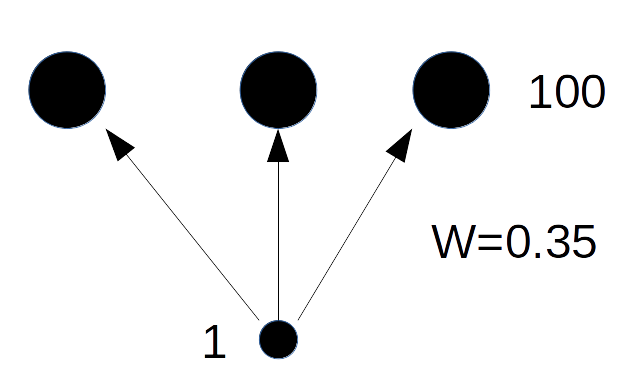
\includegraphics[scale=0.75]{P4_2.png}
\end{center}

The greedy algorithm will begin by selecting the bottom node, whose expected value is given by $f(X_b) = 3*0.35*100 + 1 = 106$. 
After that the greedy search will add one of the top nodes at each step selected at random.  

\begin{tabular}{c|c|c|c}
$f(X_i)$ & Step 1 & Step 2 & Step 3 \\
\hline
$X_{top}\ l$ & 100 & \textbf{65} & --\\
$X_{top}\ c$ & 100 & 65 & \textbf{65}\\
$X_{top}\ r$ & 100 & 65 & \ 65\\
$X_{bottom}$ & \textbf{106} & -- & --\\
\end{tabular}

The resulting score is  $f(S_3) = 236$. 

By selecting the optimal set of the three top nodes, the resulting score is $f(T) = 300$, with $ 0.8 f(T) = 0.8*300 = 240 > 236$. 
% Question 4.3
\newquestion{4.3}
A sufficient property for Greedy hill climb optimality is as follows. 
$$ f(X_i) \geq f(X_j)\ \text{for} \ j \in X_i, i \neq j $$
This states that the expected cascade size for the superset of any node should be higher than the expected cascade size for that node. Since $f(S)$ is submodular, this will guarentee that there can be no benefit of adding $N_j$ once $N_i$ is added. 
% Question 4.4
\newquestion{4.4}
Define the family to be the set of graphs where each member of the family is composed of $k$ disconnected chains of length $b$ with weight 1. So for example, $E(3)$ is a set of $k$ chains with 3 nodes. At each step, the hill climbing algorithm will have selected the root node of a chain. This is clearly the optimal solution. Then we can observe the following. 

$$ f(S_k) - f(T) + \sum_{i=1}^k \delta_i > b $$
$$ f(S_k) = f(T) = kb $$ 
$$ \delta_i = b \ \text{for} \ i \leq b, \delta_i = 0 \ \text{for} \ i > b $$ 

$$ \therefore \sum_{i=1}^k \delta_i = kb \text{for} k \leq b, \sum_{i=1}^k \delta_i = b^2 \text{for} k \geq b $$

$$ b^2 > b, \ kb >b, \text{since} \ b, k \in \mathbb{Z} $$

% Information sheet
% Fill out the information below (this should be the last page of your assignment)
\addinformationsheet
{\Large
\textbf{Your name:} John Mern\hrulefill  % Put your name here
\\
\textbf{Email:} jmern91@stanford.edu\underline{\hspace*{6cm}}  % Put your e-mail here
\textbf{SUID:} jmern91  % Put your student ID here
\\*[2ex] 
}
Discussion Group: \hrulefill   % List your study group here
\\
\vfill\vfill
I acknowledge and accept the Honor Code.\\*[3ex]
\bigskip
\textit{(Signed)}  
JM   % Replace this line with your initials
\vfill





\end{document}
